% Frame : Third Assignment
\begin{frame}
    \frametitle{Third Assignment Dataset}
    For the third assignment we are implementing a transformer which is 
    trained on the MNIST Dataset. The MNIST dataset has:
    \begin{itemize}
        \item 60,000 training images
        \item 10,000 testing images
        \item 10 classes
        \item 28x28 pixels each image
    \end{itemize}
    \begin{figure}
        \centering
        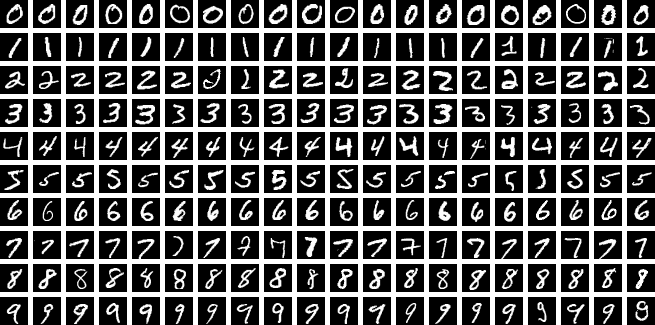
\includegraphics[height=0.4\textheight]{media/3rdAssignment/MNIST_dataset_example.png}
        \caption{MNIST Dataset}
    \end{figure}
\end{frame}

% Frame : Simple Transformer
\begin{frame}
    \frametitle{Simple Transformer}
    The simple transformer 
    \begin{itemize}
        \item 
    \end{itemize}
\end{frame}

% Frame : Seft-Attention Transformer 
\begin{frame}
    \frametitle{Self-Attention Transformer}
    The self-attention transformer 
    \begin{itemize}
        \item 
    \end{itemize}
\end{frame}

% Frame : PCA
\begin{frame}
    \frametitle{PCA}
    The PCA 
    \begin{itemize}
        \item 
    \end{itemize}
\end{frame}

% Frame : CNN Interpreter
\begin{frame}
    \frametitle{CNN Interpreter}
    The CNN Interpreter 
    \begin{itemize}
        \item 
    \end{itemize}
\end{frame}

% Frame : Custom Test Set vs MNIST Test Set
\begin{frame}
    \frametitle{Custom Test Set vs MNIST Test Set}
    The custom test set 
    \begin{itemize}
        \item 
    \end{itemize}
\end{frame}

% Frame : PCA Number of Components
\begin{frame}
    \frametitle{PCA Number of Components Demonstration}
    \begin{figure}
        \centering
        \includegraphics[height=0.4\textheight]{media/3rdAssignment/pca.png}
    \end{figure}
\end{frame}